\section{Appendix: GAMYGDALA Scalability}
The developers of GAMYGDALA did not implement all of the Software Engineering principles, because most of the time this will impact the scalability of the code. \par
During this project, the GAMYGDALA port has been refactored and some Software Engineering principles have been applied. This is why the GAMYGDALA port had to be tested to see if the refactor has any impact on the scalability. \\

The scalability was tested by calculating the execution time of the \texttt{appraise()} and the \texttt{decayAll()}. This is because those two methods are affected by the amount of entities within engine. Because there are so many entities within GAMYGDALA, the test has been split into three smaller tests. These tests differ in the amount of relations between Agents, the amount of Beliefs that have to be appraised and the amount of Goals that are affected by the Beliefs. \par
Foreach test the duration has been calculated for 1, 10, 100, 1000 and 10000 Agents with 5, 50 and 500 Goals per Agent. In the figures below, you can see the results of the tests plotted onto three different graphs. Below each graph, you can see the settings of the tests. The x- and y-axis have a logarithmic scale.

\begin{figure}[H]
  \centering
  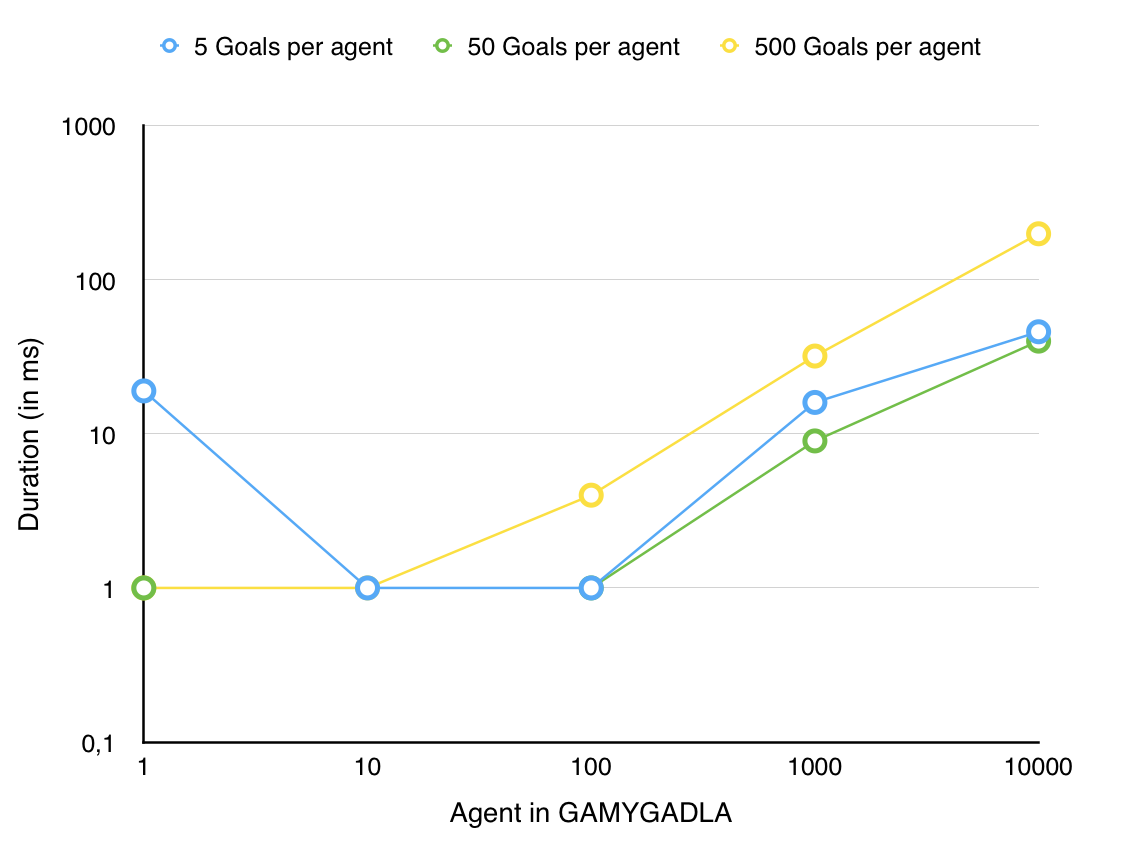
\includegraphics[scale=0.5]{scalability/1.jpg}
  \caption{Scalability, Relations: 1, Beliefs: 1 and Affected Goals: 1}
  \label{scala:first}
\end{figure}

\begin{figure}[H]
  \centering
  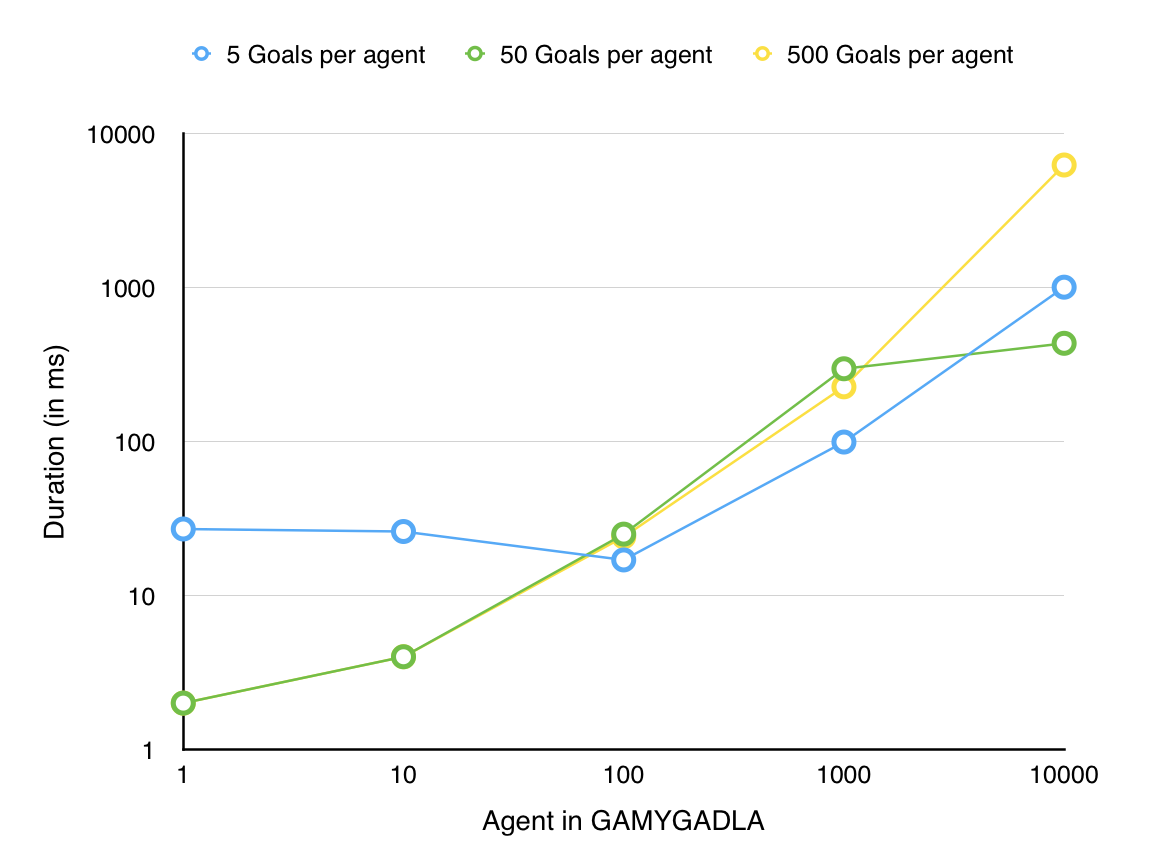
\includegraphics[scale=0.5]{scalability/2.jpg}
  \caption{Scalability, Relations: 10, Beliefs: 10 and Affected Goals: 10}
  \label{scala:second}
\end{figure}

\begin{figure}[H]
  \centering
  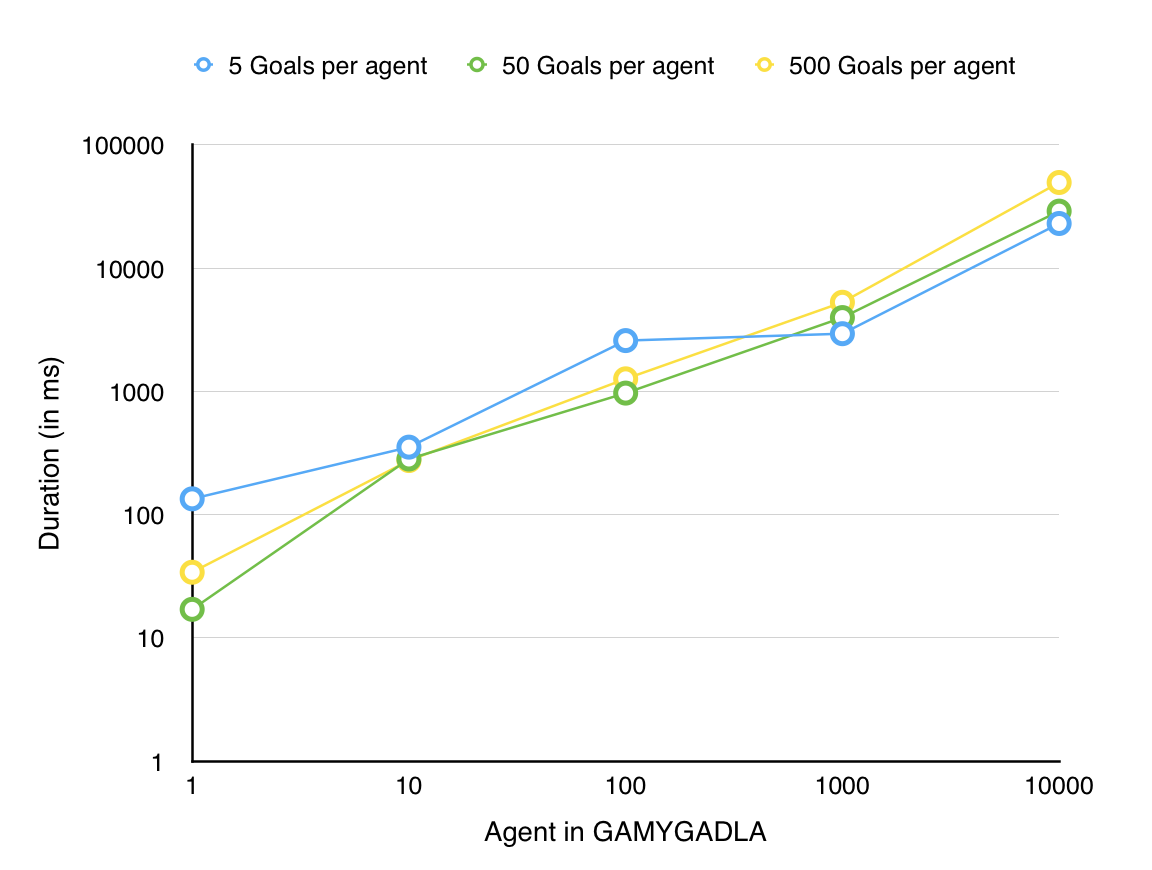
\includegraphics[scale=0.5]{scalability/3.jpg}
  \caption{Scalability, Relations: 100, Beliefs: 100 and Affected Goals: 100}
  \label{scala:third}
\end{figure}

From these graphs you can see that there is a linear relation between the amount of Agents and the execution time. From this you can conclude that the port of GAMYGDALA is scalable. At least untill 10000 Agents, 500 Goals per Agent, 100 Relations, 100 Beliefs and 100 Affected Goals. We think that this is enough, because 1000 Agents with 500 Goals is a really really big system.